\documentclass[12pt]{article}

\usepackage[brazilian]{babel}
\usepackage[utf8x]{inputenc}
\usepackage[T1]{fontenc}
\usepackage{graphicx}
\usepackage{url}
\usepackage[a4paper, top=2.5cm, bottom=2.5cm, left=1.5cm, right=1.5cm]{geometry}
\usepackage{listings}
\usepackage{color}
\usepackage{fancyhdr}
\usepackage{fancyvrb}
\usepackage{hyperref}
\usepackage{caption}
\usepackage{subcaption}
\usepackage{indentfirst}

%%%%%%%%%%%%%%%%%%%%%%%%%%%%%% DOCUMENT VARIABLES %%%%%%%%%%%%%%%%%%%%%%%%%%%%%%%%%%%%%%%
\def\doctitle{Comunicação UDP/IP}
\def\labnumber{6}
\def\fulltitle{Laboratório \labnumber -- \doctitle}
\def\docauthor{Thiago José Michelin}
\def\docsubj{Sistemas Microcomputadorizados}
\def\docsubjmn{SMC}

%%%%%%%%%%%%%%%%%%%%%%%%%%%%%% CONFIGURATION FOR GRAPHICX PACKAGE %%%%%%%%%%%%%%%%%%%%%%%
\graphicspath{{../img}}

%%%%%%%%%%%%%%%%%%%%%%%%%%%%%% COLOR CONFIGURATION FOR THE TEXT %%%%%%%%%%%%%%%%%%%%%%%%%
\definecolor{org}{RGB}{255, 102, 0}     % Orange
\definecolor{gry}{RGB}{89, 89, 89}      % Gray
\definecolor{gre}{RGB}{0, 128, 0}       % Green
\definecolor{rdy}{RGB}{204, 0, 0}       % Red
\definecolor{blu}{rgb}{0, 0.33, 0.83}   % Blue
\definecolor{pur}{RGB}{153, 0, 153}     % Purple
\definecolor{yel}{RGB}{255, 204, 0}     % Yellow
\definecolor{ros}{RGB}{255, 51, 153}    % Rose

%%%%%%%%%%%%%%%%%%%%%%%%%%%%%% CONFIGURATION FOR LISTINGS PACKAGE %%%%%%%%%%%%%%%%%%%%%%%
\definecolor{backcolor}{RGB}{255, 255, 255}
\definecolor{strings}{RGB}{153, 102, 51}
\definecolor{comments}{rgb}{0.25, 0.5, 0.35}
\definecolor{keywords}{rgb}{0.5, 0, 0.35}
\definecolor{lstnumbers}{RGB}{80, 80, 80}
\definecolor{codecolor}{RGB}{64, 64, 64}

\lstdefinestyle{circ_style}{
  backgroundcolor=\color{backcolor},
  commentstyle=\color{comments},
  keywordstyle=\color{keywords},
  numberstyle=\tiny\color{lstnumbers},
  stringstyle=\color{strings},
  basicstyle=\scriptsize\ttfamily\color{codecolor},
  breakatwhitespace=false,
  breaklines=true,
  captionpos=t,
  keepspaces=true,
  numbers=left,
  showspaces=false,
  showstringspaces=false,
  showtabs=false,
  tabsize=2,
  frame=single
}

\lstset{style=circ_style}

\lstset{literate=
  {á}{{\'a}}1 {é}{{\'e}}1 {í}{{\'i}}1 {ó}{{\'o}}1 {ú}{{\'u}}1
  {Á}{{\'A}}1 {É}{{\'E}}1 {Í}{{\'I}}1 {Ó}{{\'O}}1 {Ú}{{\'U}}1
  {à}{{\`a}}1 {è}{{\`e}}1 {ì}{{\`i}}1 {ò}{{\`o}}1 {ù}{{\`u}}1
  {À}{{\`A}}1 {È}{{\'E}}1 {Ì}{{\`I}}1 {Ò}{{\`O}}1 {Ù}{{\`U}}1
  {ä}{{\"a}}1 {ë}{{\"e}}1 {ï}{{\"i}}1 {ö}{{\"o}}1 {ü}{{\"u}}1
  {Ä}{{\"A}}1 {Ë}{{\"E}}1 {Ï}{{\"I}}1 {Ö}{{\"O}}1 {Ü}{{\"U}}1
  {â}{{\^a}}1 {ê}{{\^e}}1 {î}{{\^i}}1 {ô}{{\^o}}1 {û}{{\^u}}1
  {Â}{{\^A}}1 {Ê}{{\^E}}1 {Î}{{\^I}}1 {Ô}{{\^O}}1 {Û}{{\^U}}1
  {ã}{{\~a}}1 {Ã}{{\~A}}1
  {ß}{{\ss}}1 {ç}{{\c c}}1 {Ç}{{\c C}}1
}

%%%%%%%%%%%%%%%%%%%%%%%%%%%%%% CONFIGURATION FOR HYPERREF PACKAGE %%%%%%%%%%%%%%%%%%%%%%%
\hypersetup{
  colorlinks=true,
  breaklinks=true,
  linkcolor=red,
  citecolor=red,
  urlcolor=blu,
  pdftitle={\fulltitle},
  pdfauthor={\docauthor}
}

%%%%%%%%%%%%%%%%%%%%%%% CONFIGURATION FOR FANCY HEADER AND FOOTER PACKAGES %%%%%%%%%%%%%%
\pagestyle{fancy}
\fancyhf{}
\setlength{\headheight}{15pt}
\rhead{\docsubjmn}
\lhead{\docsubj}
\cfoot{\thepage}

\renewcommand{\lstlistingname}{Bloco de código}
\newcommand{\bc}[1]{Bloco de Código \ref{#1}}
\newcommand{\ebt}[2]{\textcolor{#1}{\texttt{#2}}}
\newcommand{\ebf}[2]{\textcolor{#1}{\textbf{#2}}}

\title{\doctitle}
\author{\docauthor}

\makeatletter
\makeatother

\begin{document}

%%%%%%%%%%%%%%%%%%%%%%%%%%%%%%%%%%%%%%%%%%%%%%%%%%%%%%%%%%%%%%%%%%%%%%%%%%%%%%%%%%%%%%%%%

\begin{titlepage}
  \centering
  \vspace*{0.5 cm}
  
\includegraphics[scale = 0.5]{logo_unesp.pdf}\\[2.0 cm] % University Logo
  \textsc{\large Faculdade de Engenharia e Ciências de Guaratinguetá}\\[0.3cm]
  \textsc{\large Departamento de Engenharia Elétrica}\\[3.0cm]
  { \LARGE \bfseries \docsubj }\\

  \vspace{5cm}

  \textsc{\large Laboratório \labnumber}\\
  \vspace{1cm}
  \textsc{\large \doctitle}

\end{titlepage}

%%%%%%%%%%%%%%%%%%%%%%%%%%%%%%%%%%%%%%%%%%%%%%%%%%%%%%%%%%%%%%%%%%%%%%%%%%%%%%%%%%%%%%%%%

{
  \hypersetup{hidelinks}
  \tableofcontents
}

\newpage

%%%%%%%%%%%%%%%%%%%%%%%%%%%%%%%%%%%%%%%%%%%%%%%%%%%%%%%%%%%%%%%%%%%%%%%%%%%%%%%%%%%%%%%%%

\section{Objetivos}

\begin{itemize}
  \item Estudar e implementar a comunicação UDP/IP entre diferentes dispositivos de
    uma rede.
\end{itemize}

\section{O Protocolo UDP}

O conjunto de protocolos da Internet admite um protocolo de transporte não orientado
a conexões, o protocolo de datagrama do usuário, ou \textbf{UDP} (\textit{User
Datagram Protocol}). O UDP oferece um meio para as aplicações enviarem datagramas IP
encapsulados sem que seja necessário estabelecer uma conexão.

O UDP transmite \textbf{segmentos} que consistem em um cabeçalho de 8 bytes, seguido
pela carga útil (\textit{payload}). O cabeçalho é mostrado na Figura \ref{fig:udpheader}.
Os dois números de \textbf{portas} servem para identificar processos nas máquinas de
origem e destino. Quando um pacote UDP é recebido, sua carga útil é entregue ao processo
associado à porta de destino. Essa associação ocorre quando a primitiva \texttt{BIND},
ou algo semelhante, é utilizada. Pense nas portas como caixas de correio que as aplicações
podem utilizar para receber pacotes. De fato, a principal vantagem em utilizar o UDP em
relação ao uso do IP bruto é a adição das portas de origem e destino. Sem os campos de
números de portas, a camada de transporte não saberia o que fazer como pacote recebido.
Com eles, a camada entrega o segmento encapsulado à aplicação correta.

\begin{figure}[ht]
  \centering
  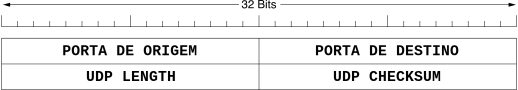
\includegraphics[width=.9\textwidth]{udpheader.pdf}
  \caption{Cabeçalho UDP \cite{tanembaum2021}.}
  \label{fig:udpheader}
\end{figure}

A porta de origem é necessária, principalmente, quando uma resposta precisa ser enviada
de volta à origem. Copiando o campo \texttt{PORTA DE ORIGEM} do segmento de entrada no
campo \texttt{PORTA DE DESTINO} do segmento de saída, o processo que transmite a
resposta pode especificar qual processo na máquina transmissora deve recebê-lo.

O campo \texttt{UDP LENGTH} inclui o cabeçalho de 8 bytes e os dados. O comprimento
mínimo é de 8 bytes, para incluir o cabeçalho. O comprimento máximo é de 65.515 bytes,
que é menor que o maior número que caberá em 16 bits, devido ao limite de tamanho nos
pacotes IP.

Um campo opcional de \texttt{UDP CHECKSUM} também é fornecido para gerar confiabilidade
extra. Ele faz o \textit{checksum} do cabeçalho, dos dados e de um pseudocabeçalho
conceitual do IP. Ao realizar um cálculo, o campo de \textit{checksum} é definido como
zero e o campo de dados é preenchido com um byte zero adicional se seu comprimento for
um número ímpar. O algoritmo de checksum consiste, simplesmente, em somar todas as
palavras de 16 bits com complemento de um e apanhar o complemento de um da soma. Por
conseguinte, quando o receptor realizar o cálculo sobre o segmento inteiro, incluindo
o campo de \textit{Checksum}, o resultado deve ser 0. Se o checksum não for calculado,
ele será armazenado como zero, pois, por uma feliz coincidência da aritmética de
complemento de um, um valor 0 verdadeiro calculado é armazenado com todos os bits iguais
a 1. É tolice desativá-lo, a menos que a qualidade dos dados não tenha importância
(por exemplo, no caso de voz digitalizada).

Vale a pena mencionar algumas ações que o UDP \textbf{não} realiza. Ele não realiza
controle de fluxo, controle de congestionamento ou retransmissão após a recepção de
um segmento incorreto. Tudo isso cabe aos processos do usuário. O que ele faz é
fornecer uma interface para o protocolo IP com o recurso adicional de demultiplexação
de vários processos que utilizam as portas e detecção opcional de erro fim a fim
\cite{tanembaum2021}.

\section{Programação em C usando Sockets e o protocolo UDP}

Os programas cliente e servidor utilizando sockets e o protocolo UDP são bastante
similares em relação às suas versões utilizando o protocolo TCP, conforme vimos no
laboratório anterior. A grande diferença é que, neste caso, não utilizaremos as intruções
para estabelecer uma conexão entre os dois \textit{hosts}, além de alguns parâmetros
diferentes que são utilizados durante a chamada ao método \texttt{socket()}.

\subsection{Passos para a criação do socket no lado do cliente}

A criação de um socket no lado cliente envolve, basicamente, 2 passos, conforme enumerado
abaixo e ilustrado pela Figura \ref{fig:client_diagram}.

\begin{itemize}
  \item[1.] Criar um socket com a chamada ao sistema \texttt{socket()} \cite{man_socket}.
  \item[2.] Enviar e receber dados utilizando as funções \texttt{sendto()} \cite{man_send}
    e \texttt{recvfrom()} \cite{man_recv}.
\end{itemize}

\subsubsection{Passos para a criação do socket no lado do servidor}

De forma semelhante, a criação do socket no lado servidor emprega os passos enumerados
abaixo e ilustrados pela figura \ref{fig:server_diagram}.

\begin{itemize}
  \item[1.] Criar um socket com a chamada ao sistema \texttt{socket()} \cite{man_socket}.
  \item[2.] Vincular o socket a um endereço utilizando a função \texttt{bind()}
    \cite{man_bind}.
  \item[3.] Enviar e receber dados usando as funções \texttt{sendto()} e
    \texttt{recvfrom()}.
\end{itemize}

\begin{figure}[h]
  \centering
  \begin{subfigure}[b]{0.48\textwidth}
    \centering
    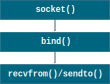
\includegraphics[width=0.6\textwidth]{socket_server_diagram.pdf}
    \caption{Diagrama para o servidor.}
    \label{fig:server_diagram}
  \end{subfigure}
    \hfill
  \begin{subfigure}[b]{0.48\textwidth}
    \centering
    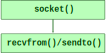
\includegraphics[width=0.6\textwidth]{socket_client_diagram.pdf}
    \caption{Diagrama para o cliente.}
    \label{fig:client_diagram}
  \end{subfigure}
  \caption{Diagramas para a construção do socket utilizando o protocolo UDP.}
\end{figure}

\newpage

\section{Exemplo de Programação}

Neste exemplo de programação, assim como no laboratório anterior, vamos criar os
processos \texttt{echoserver} (servidor) e \texttt{udpclient} (cliente). A diferença é
que, desta vez, faremos uso do protocolo UDP ao invés do protocolo TCP.

\subsection{Arquivo de cabeçalho com definições comuns}

Um arquivo de cabeçalho, denominado ``\texttt{defs.h}'', que possui algumas definições
comuns tanto ao cliente quanto ao servidor, foi criado separadamente dos demais arquivos
de forma a facilitar o desenvolvimento. Este arquivo foi salvo em um diretório chamado
\texttt{include}.

\lstinputlisting[language=C++, caption={Arquivo de cabeçalho \texttt{defs.h}.}]
  {../programs/include/defs.h}

\subsection{Servidor para Linux}

O código utilizado para implementar o servidor foi dividido em três arquivos.

\subsubsection{Arquivo de código-fonte \texttt{udpserver.c}}

\lstinputlisting[language=C++]{../programs/udpserver/udpserver.c}

\subsubsection{Arquivo de código-fonte \texttt{echoserver.h}}

\lstinputlisting[language=C++]{../programs/udpserver/echoserver.h}

\subsubsection{Arquivo de código-fonte \texttt{echoserver.c}}

\lstinputlisting[language=C++]{../programs/udpserver/echoserver.c}

\subsubsection{Arquivo \texttt{Makefile}}

\lstinputlisting[language=make]{../programs/udpserver/Makefile}

\subsection{Cliente para Linux}

De forma similar ao servidor, o código para implementar o cliente também foi
dividido em três arquivos.

\subsubsection{Arquivo de código-fonte \texttt{udpclient.c}}

\lstinputlisting[language=C++]{../programs/udpclient/udpclient.c}

\subsubsection{Arquivo de código-fonte \texttt{messageclient.h}}

\lstinputlisting[language=C++]{../programs/udpclient/messageclient.h}

\subsubsection{Arquivo de código-fonte \texttt{messageclient.c}}

\lstinputlisting[language=C++]{../programs/udpclient/messageclient.c}

\subsubsection{Arquivo \texttt{Makefile}}

\lstinputlisting[language=make]{../programs/udpclient/Makefile}

\subsection{Servidor para Windows}

O código apresentado abaixo é utilizado para implementar um servidor para Windows.
Repare que algumas chamadas às funções do sistema são um pouco diferentes daquelas
utilizadas no cliente para Linux e refletem a utilização de bibliotecas específicas
de cada plataforma.

\subsubsection{Arquivo de código-fonte \texttt{udpserver.c}}

\lstinputlisting[language=C++]{../programs/udpserverwin/udpserver.c}

\subsubsection{Arquivo de código-fonte \texttt{echoserver.h}}

\lstinputlisting[language=C++]{../programs/udpserverwin/echoserver.h}

\subsubsection{Arquivo de código-fonte \texttt{echoserver.c}}

\lstinputlisting[language=C++]{../programs/udpserverwin/echoserver.c}

\subsubsection{Arquivo Makefile}

\lstinputlisting[language=make]{../programs/udpserverwin/Makefile}

\subsection{Cliente para Windows}

De forma similar ao servidor para Windows, o cliente também apresenta algumas
diferenças em relação ao código para Linux.

\subsubsection{Arquivo de código-fonte \texttt{udpclient.c}}

\lstinputlisting[language=C++]{../programs/udpclientwin/udpclient.c}

\subsubsection{Arquivo de código-fonte \texttt{messageclient.h}}

\lstinputlisting[language=C++]{../programs/udpclientwin/messageclient.h}

\subsubsection{Arquivo de código-fonte \texttt{messageclient.c}}

\lstinputlisting[language=C++]{../programs/udpclientwin/messageclient.c}

\subsubsection{Arquivo Makefile}

\lstinputlisting[language=make]{../programs/udpclientwin/Makefile}

%%%%%%%%%%%%%%%%%%%%%%%%%%%%%%%%%%%%%%%%%%%%%%%%%%%%%%%%%%%%%%%%%%%%%%%%%%%%%%%%%%%%%%%%%

\newpage
\bibliographystyle{ieeetr}
\bibliography{../ref/ref.bib}

\end{document}
